%!TEX program = xelatex
\documentclass{article}
\usepackage{LaTeX-Submodule/template}

% Additional packages & macros
\usepackage{multicol} % Use multiple columns
\usepackage{textcomp, upquote} % Code block quotations support 

% Header and footer
\newcommand{\unitName}{Engineering Computation}
\newcommand{\unitTime}{Semester 2, 2021}
\newcommand{\unitCoordinator}{Dr Michael Dallaston}
\newcommand{\documentAuthors}{\textsc{Tarang Janawalkar}}

\fancyhf{}
\fancyhead[L]{\unitName}
\fancyhead[R]{\leftmark}
\fancyfoot[C]{\thepage}

% Copyright
\usepackage[
    type={CC},
    modifier={by-nc-sa},
    version={4.0},
    imagewidth={5em},
    hyphenation={raggedright}
]{doclicense}

\date{}

\begin{document}
%
\begin{titlepage}
    \vspace*{\fill}
    \begin{center}
        \LARGE{\textbf{\unitName}} \\[0.1in]
        \normalsize{\unitTime} \\[0.2in]
        \normalsize\textit{\unitCoordinator} \\[0.2in]
        \documentAuthors{}
    \end{center}
    \vspace*{\fill}
    \doclicenseThis
    \thispagestyle{empty}
\end{titlepage}
\newpage
%
\tableofcontents
\newpage
%
\lstset{language=Matlab, upquote=true}
\lstset{morekeywords={randi, false, imshow, drawpolygon, polyarea, drawline, ones, imread, VideoWriter, XData, YData, getFrame, writeVideo, deg2rad, soundsc, resample, audiowrite, sind, fitlm}}
%
\section{MATLAB Functions}
\begin{table}[H]
    \centering
    \begin{tabular}{c c}
        \toprule
        Function Syntax         & Function Output                \\
        \midrule
        \lstinline!y = sin(x)!  & Sine with \(x\) in radians.    \\
        \lstinline!y = sind(x)! & Sine with \(x\) in degrees.    \\
        \lstinline!y = asin(x)! & Arcsine with \(y\) in radians. \\
        \lstinline!y = exp(x)!  & \(e^x\).                       \\
        \lstinline!y = log(x)!  & \(\ln{\left( x \right)}\).     \\
        \bottomrule
    \end{tabular}
    \caption{Common mathematical functions in MATLAB.}
\end{table}
All the above functions are element-wise.
\begin{table}[H]
    \centering
    \begin{tabular}{c c}
        \toprule
        Function Syntax                   & Function Output(s)                                                 \\
        \midrule
        \lstinline!A = zeros(m, n)!       & Creates an \(m \times n\) matrix containing zeros.                 \\
        \lstinline!A = ones(m, n)!        & Creates an \(m \times n\) matrix containing ones.                  \\
        \lstinline!I = eye(m)!            & Creates an \(m \times m\) identity matrix.                         \\
        \lstinline!a = linspace(a, b, x)! & Creates an evenly spaced vector with bounds \(\left[a, b\right]\). \\
        \lstinline!y = length(A)!         & The largest dimension of \(A\).                                    \\
        \lstinline![m, n] = size(A)!      & The dimensions of \(A\).                                           \\
        \lstinline!y = min(a)!            & The minimum value in the vector \(a\).                             \\
        \lstinline!y = max(a)!            & The maximum value in the vector \(a\).                             \\
        \bottomrule
    \end{tabular}
    \caption{Matrices and arrays in MATLAB.}
\end{table}
When manipulating matrices, \verb!*!, \verb!^!, perform matrix operations, while prepending an operator with a dot (\verb!.!) performs an element-wise operation.
\subsection{Plotting}
\begin{table}[H]
    \centering
    \begin{tabular}{c c}
        \toprule
        Function Syntax                   & Function Output(s)                                                      \\
        \midrule
        \lstinline!plot(x, y)!            & Plots given \(x\) and \(y\) coordinate vectors.                         \\
        \lstinline!fplot(@f, [a, b])!     & Plots the anonymous function over the domain \(\left[ a,\: b \right]\). \\
        \lstinline!title('string')!       & Adds title to current plot.                                             \\
        \lstinline!xlabel('string')!      & Adds \(x\)-axis label to current plot.                                  \\
        \lstinline!ylabel('string')!      & Adds \(y\)-axis label to current plot.                                  \\
        \lstinline!legend('string1',...)! & Adds legend to plot.                                                    \\ % chktex 11
        \lstinline!figure!                & Creates a new figure.                                                   \\
        \bottomrule
    \end{tabular}
    \caption{Plotting in MATLAB.}
    % \label{}
\end{table}
\subsection{Operations in MATLAB}
\subsubsection{Conditional Operations}
\begin{multicols}{2}
    \begin{lstlisting}
if expression
    statements
else if expression
    statements
else
    statements
end
    \end{lstlisting}
    \columnbreak
    Code inside an \lstinline{if} statement only executes if the expression is true. Note that only one branch will execute depending on which expression is true.
\end{multicols}
\subsubsection{Iterative Operations}
\begin{multicols}{2}
    \begin{lstlisting}
while expression
    statements
end
    \end{lstlisting}
    \columnbreak
    Statements inside a \lstinline{while} loop repeat while the expression is true.
\end{multicols}
\begin{multicols}{2}
    \begin{lstlisting}
for index = values
    statements
end
    \end{lstlisting}
    \columnbreak
    Statements inside a \lstinline{for} loop execute a specific number of times, based on the length of \lstinline{values}.
\end{multicols}
\section{Differential Equations}
\begin{definition}
    A differential equation is an equation that involves the derivatives of a function as well as the function itself.
    An ordinary differential equation (ODE) is a differential equation of a function with only one independent variable.
\end{definition}
\subsection{Electrical Systems}
\begin{theorem}[VI Relationship between Resistors]
    \begin{equation*}
        v = i R
    \end{equation*}
\end{theorem}
\begin{theorem}[VI Relationship between Inductors]
    \begin{equation*}
        v = L \dv{i}{t}
    \end{equation*}
\end{theorem}
\begin{theorem}[VI Relationship between Capacitors]
    \begin{equation*}
        i = C \dv{v}{t}
    \end{equation*}
\end{theorem}
\begin{theorem}[Kirchhoff's Voltage Law]
    The sum of all voltages around a loop equals zero.
    \begin{equation*}
        \sum v_{\mathrm{loop}} = 0
    \end{equation*}
\end{theorem}
\begin{theorem}[Kirchhoff's Current Law]
    The sum of all currents into a node equals zero.
    \begin{equation*}
        \sum i_{\mathrm{node}} = 0
    \end{equation*}
\end{theorem}
\subsection{Mechanical Systems}
\begin{theorem}[Newton's Second Law]
    \begin{equation*}
        \sum F = \dv{p}{t}
    \end{equation*}
    where \(p = mv\).
\end{theorem}
\begin{theorem}[Thrust Force]
    \begin{equation*}
        F_T = (c - v) d_f
    \end{equation*}
\end{theorem}
\begin{theorem}[Force of Gravity]
    \begin{equation*}
        F_g = mg
    \end{equation*}
\end{theorem}
\begin{theorem}[Force of a Spring]
    \begin{equation*}
        F = -kx
    \end{equation*}
\end{theorem}
\section{First-Order Ordinary Differential Equations}
\subsection{Separable ODEs}
\begin{equation*}
    \dv{y}{t} = F(y,\: t)
\end{equation*}
\begin{enumerate}
    \item Rewrite the equation in the form: \(f(y)\dd{y} = g(t)\dd{t}\).
    \item Integrate both sides: \(\int f(y)\dd{y} = \int g(t)\dd{t}\).
    \item Rearrange for the explicit form of \(y(t)\).
\end{enumerate}
\subsection{Linear ODEs}
Let \(P=P(t)\), \(Q=Q(t)\) and \(\mu = \mu(t)\)
\begin{equation*}
    \dv{y}{t} + Py = Q
\end{equation*}
\begin{enumerate}
    \item Determine the integrating factor: \(\displaystyle \mu=\exp{\left( \int P \dd{t} \right)}\).
    \item Solve:
          \begin{equation*}
              y=\frac{1}{\mu}\left(\int Q \mu \dd{t} + C\right)
          \end{equation*}
\end{enumerate}
\begin{proof}
    To solve a first-order linear differential equation, determine an integrating factor \(\mu = \mu(t)\) such that
    \begin{equation}
        P \mu = \dv{\mu}{t} \label{eq:integrating_factor}
    \end{equation}
    Multiplying the equation by \(\mu \) gives
    \begin{align*}
        \mu \dv{y}{t} + P \mu y             & = Q \mu                                           \\
        \mu \dv{y}{t} + \dv{\mu}{t} y       & = Q \mu                                           \\
        \dv{t}\bigl(\mu y\bigr)             & = Q \mu                                           \\
        \int \dv{t}\bigl(\mu y\bigr) \dd{t} & = \int Q \mu \dd{t}                               \\
        \mu y                               & = \int Q \mu \dd{t}                               \\
        y                                   & = \frac{1}{\mu}\left(\int Q \mu \dd{t} + C\right)
    \end{align*}
    To determine \(\mu \) we can rearrange \hyperref[eq:integrating_factor]{Equation~\ref{eq:integrating_factor}} into
    \begin{align*}
        P = \frac{1}{\mu}\dv{\mu}{t}
    \end{align*}
    By recognition, this is the derivative of the natural logarithm of \(\mu \) with respect to \(t\).
    \begin{align*}
        P             & = \dv{t}(\ln{\left( \mu \right)})                       \\
        \int P \dd{t} & = \int \dv{t}\bigl(\ln{\left( \mu \right)}\bigr) \dd{t} \\
        \int P \dd{t} & = \ln{\left( \mu \right)}                               \\
        \mu           & = \exp{\left( \int P \dd{t} \right)}
    \end{align*}
\end{proof}
\subsection{Solution using Linearisation}
A function can be linearised by using its 1st degree Taylor polynomial near \(a\).
\begin{equation*}
    f(x) \approx f(a) + f'(a)(x-a) + \mathcal{O}(x^2)
\end{equation*}
This new polynomial can be substituted to form a linear ODE, which can be solved using an integrating factor.
\newpage
\section{Second-Order Ordinary Differential Equations}
\subsection{Constant Coefficient Linear ODEs}
\begin{equation*}
    a \dv[2]{y}{t} + b \dv{y}{t} + c y = Q(t)
\end{equation*}
where \(a,\:b,\:c\) are constants.
\subsection{Linearity of Solutions}
\begin{theorem}[Principle of Superposition]\label{theorem:superposition}
    As the given ODE is linear, if \(y_1(t)\) is a solution to the equation
    \begin{equation*}
        a \dv[2]{y_1}{t} + b \dv{y_1}{t} + cy_1 = Q_1(t)
    \end{equation*}
    and \(y_2(t)\) is a solution to
    \begin{equation*}
        a \dv[2]{y_2}{t} + b \dv{y_2}{t} + cy_2 = Q_2(t)
    \end{equation*}
    then for the function \(y = c_1y_1+c_2y_2\)
    \begin{equation*}
        a \dv[2]{y}{t} + b \dv{y}{t} + cy = c_1Q_1(t) + c_2Q_2(t)
    \end{equation*}
    where \(c_1\) and \(c_2\) are constants.
\end{theorem}
% \begin{proof}
% \begin{align*}
%     a \dv[2]{y}{t} + b \dv{y}{t} + cy &= a \dv[2]{t}(k_1y_1+k_2y_2) + b \dv{t}(k_1y_1+k_2y_2) + c(k_1y_1+k_2y_2) \\
%     &= k_1\left( a \dv[2]{y}{t} + b \dv{y}{t} + cy \right)a \dv[2]{t}(k_1y_1+k_2y_2) + b \dv{t}(k_1y_1+k_2y_2) + c(k_1y_1+k_2y_2) \\
% \end{align*}
% \end{proof}
\subsection{Homogeneous ODEs}
\begin{definition}
    A homogeneous ODE has \(Q(t)=0\), which gives
    \begin{equation*}
        a \dv[2]{y}{t} + b \dv{y}{t} + c y = 0
    \end{equation*}
\end{definition}
This differential equation has a solution of the form:
\begin{equation*}
    y_H = e^{rt}
\end{equation*}
\subsection{Characteristic Equation}
By making the substitution \(y=e^{rt}\), we get
\begin{align*}
    a \dv[2]{y_H}{t} + b \dv{y_H}{t} + c y_H & = 0 \\
    ar^2e^{rt} + bre^{rt} + ce^{rt}          & = 0 \\
    (ar^2 + br + c)e^{rt}                    & = 0 \\
    ar^2 + br + c                            & = 0
\end{align*}
This is known as the characteristic or \textit{auxiliary} equation. The next step is to calculate the roots of the equation.
\begin{description}
    \item[Real Distinct Roots.] If \(b^2 > 4ac\).
    \item[Real Repeated Roots.] If \(b^2 = 4ac\).
    \item[Complex Conjugate Roots.] If \(b^2 < 4ac\).
\end{description}
\subsubsection{Real Distinct Roots}
Given \(r_1\) and \(r_2\) are real and distinct:
\begin{align*}
    y_1(t) = e^{r_1t} &  & y_2(t) = e^{r_2t}
\end{align*}
Hence the solution to the homogeneous equation is given by:
\begin{equation*}
    y_H(t) = c_1e^{r_1t} + c_2e^{r_2t}
\end{equation*}
\subsubsection{Real Repeated Roots}
Given \(r\) is a repeated root:
\begin{align*}
    y_1(t) = e^{rt} &  & y_2(t) = te^{rt}
\end{align*}
Hence the solution to the homogeneous equation is given by:
\begin{equation*}
    y_H(t) = c_1e^{rt} + c_2te^{rt}
\end{equation*}
\subsubsection{Complex Conjugate Roots}
Given \(r_1 = \alpha + \beta i\) and \(r_2 = \alpha - \beta i\) are complex conjugates:
\begin{align*}
    y_1(t) = e^{r_1t} &  & y_2(t) = e^{r_2t}
\end{align*}
Hence the solution to the homogeneous equation is given by:
\begin{equation*}
    y_H(t) = c_1e^{\alpha t}\cos{\left( \beta t \right)} + c_2e^{\alpha t}\sin{\left( \beta t \right)}
\end{equation*}
\subsection{Nonhomogeneous ODE}
A nonhomogeneous differential equation is of the form
\begin{equation*}
    a \dv[2]{y}{t} + b \dv{y}{t} + c y = Q(t)
\end{equation*}
where \(Q(t)\neq 0\).
\subsection{General Solution of a Nonhomogeneous ODE}
Recall that the solutions to any linear ODE are additive, so that if a solution \(y_P\) satisfies
the nonhomogeneous ODE, and \(y_H\) satisfies the homogeneous ODE,
\begin{equation*}
    y = y_H + y_P
\end{equation*}
must also satisfy the ODE\@.
\subsection{Undetermined Coefficients}
To solve for \(y_P\), we substitute a guess, and
determined the coefficients from the ODE itself.

The particular solution will depend on what \(Q(t)\) looks like.
\begin{table}[H]
    \centering
    \begin{tabular}{c c}
        \toprule
        \(Q(t)\)                                                          & \(y_P\)                                                             \\
        \midrule
        a constant                                                        & \(A\)                                                               \\
        \(n\)th degree polynomial                                         & \(A_0 + A_1t + \cdots + A_{n-1}t^{n-1} + A_n t^n\)                  \\
        \(e^{\alpha t}\)                                                  & \(Ae^{\alpha t}\)                                                   \\
        \(\cos{\left( \alpha t \right)}\)                                 & \(A\cos{\left( \alpha t \right)} + B\sin{\left( \alpha t \right)}\) \\
        \(\sin{\left( \alpha t \right)}\)                                 & \(A\cos{\left( \alpha t \right)} + B\sin{\left( \alpha t \right)}\) \\
        \(\cos{\left( \alpha t \right)} + \sin{\left( \alpha t \right)}\) & \(A\cos{\left( \alpha t \right)} + B\sin{\left( \alpha t \right)}\) \\
        \bottomrule
    \end{tabular}
    \caption{Particular solutions for undetermined coefficients.}
    % \label{}
\end{table}
\subsection{Special Forms}
\subsubsection{Product of Forms}
If \(Q(t)\) is a product of the functions shown above, then the
particular solutions are also multiplied together and any coefficients are simplified.
\subsubsection{Sum of Forms}
If \(Q(t)\) is a sum of the functions shown above, then the
particular solutions are also added together.
\subsubsection{Linearly Dependent Case}
If \(Q(t)\) is similar to any homogenous solution, then by \textit{definition} of
a homogeneous solution, the solution will be \(0\). Hence, \(y_P\) must be multiplied by \(t\)
to ensure that the particular solution is linearly independent to the homogeneous solutions,
in order to form a \textit{fundamental set of solutions}.
\subsection{Solving the Particular Solution}
\begin{enumerate}
    \item Solve \(y_H\)
    \item Find an appropriate form for \(y_P\)
    \item Ensure that \(y_P\) is linearly independent to the homogeneous solutions
    \item Substitute \(y_P\) into the nonhomogeneous ODE and solve for the undetermined coefficients
    \item Find the general solution \(y = y_H + y_P\)
    \item Apply initial conditions
\end{enumerate}
\section{Systems of Ordinary Differential Equations}
A first-order system of differential equations has the form
\begin{equation*}
    \left \{
    \setlength\arraycolsep{0pt}
    \begin{array}{ c >{{}}c<{{}} c >{{}}c<{{}} c >{{}}c<{{}} c >{{}}c<{{}} c  }
        x'_1               & = & a_{11}x_1                         & + & a_{12}x_2                         & + & \cdots & + & a_{1n}x_n                         \\
        x'_2               & = & a_{21}x_1                         & + & a_{22}x_2                         & + & \cdots & + & a_{2n}x_n                         \\
        \vdotswithin{x'_3} &   & \vdotswithin{a_{31}}\phantom{x_1} &   & \vdotswithin{a_{32}}\phantom{x_2} &   &        &   & \vdotswithin{a_{3n}}\phantom{x_n} \\
        x'_n               & = & a_{n1}x_1                         & + & a_{n2}x_2                         & + & \cdots & + & a_{nn}x_n
    \end{array}
    \right.
\end{equation*}
where \(x_1=x_1(t),\: x_2=x_2(t),\: \dots,\: x_n=x_n(t)\) are the
functions to be determined. In matrix form, the system can be written as
\begin{align*}
    \dv{t} \begin{bmatrix}
               x_1 \\ x_2 \\ \vdots \\ x_n
           \end{bmatrix} & = \begin{bmatrix}
                                 a_{11} & a_{12} & \cdots & a_{1n} \\
                                 a_{21} & a_{22} & \cdots & a_{2n} \\
                                 \vdots & \vdots &        & \vdots \\
                                 a_{n1} & a_{n2} & \cdots & a_{nn}
                             \end{bmatrix} \begin{bmatrix}
                                               x_1 \\ x_2 \\ \vdots \\ x_n
                                           \end{bmatrix} \\
    \symbf{x}'                  & = \symbfit{A} \symbf{x}
\end{align*}
\subsection{Higher-Order ODEs}
A higher-order linear differential equation can be solved by first converting it to a first-order linear
system. Consider the \(n\)th-order homogeneous differential equation
\begin{equation*}
    y^{\left( n \right)} + a_1 y^{\left( n-1 \right)} + \cdots + a_{n-1} y' + a_n y = 0
\end{equation*}
Let
\begin{align*}
    x_1 & = y                      \\
    x_2 & = y'                     \\
        & \vdotswithin{=}          \\
    x_n & = y^{\left( n-1 \right)}
\end{align*}
so that \(\symbfit{x}=\begin{bmatrix}x_1 & x_2 & \cdots & x_n\end{bmatrix}^\top \). Then the differential equation can
be expressed as the following first-order linear system of differential equations
\begin{equation*}
    \dv{t} \begin{bmatrix}
        x_1               \\
        x_2               \\
        \vdotswithin{x_3} \\
        x_n
    \end{bmatrix} = \begin{bmatrix}
        0      & 1        & 0        & \cdots & 0      \\
        0      & 0        & 1        & \cdots & 0      \\
        \vdots & \vdots   & \vdots   & \ddots & \vdots \\
        0      & 0        & 0        & \cdots & 1      \\
        -a_n   & -a_{n-1} & -a_{n-2} & \cdots & -a_1
    \end{bmatrix} \begin{bmatrix}
        x_1               \\
        x_2               \\
        \vdotswithin{x_3} \\
        x_n
    \end{bmatrix}
\end{equation*}
\subsection{Solution Form}
Like the homogeneous case, we will guess a solution of the form
\begin{equation*}
    \symbf{x} = \symbf{q}e^{\lambda t}
\end{equation*}
which allows for the following substitution
\begin{align*}
    \lambda \symbf{q}e^{\lambda t}                                         & = \symbfit{A} \symbf{q}e^{\lambda t} \\
    \symbfit{A} \symbf{q}e^{\lambda t} - \lambda \symbf{q}e^{\lambda t}    & = \symbf{0}                          \\
    \left( \symbfit{A} - \lambda\symbfit{I} \right) \symbf{q}e^{\lambda t} & = \symbf{0}                          \\
    \left( \symbfit{A} - \lambda\symbfit{I} \right) \symbf{q}              & = \symbf{0}
\end{align*}
This equation has the trivial solution \(\symbf{q}=\symbf{0}\), however for a fundamental set of solutions,
we must let \(\symbfit{A} - \lambda\symbfit{I}\) be singular.
\subsubsection{Characteristic Equation}
To determine the eigenvalues \(\lambda \) of the matrix \(\symbf{A}\), we must solve the characteristic equation
associated with the system of ODEs. Namely,
\begin{equation*}
    \det{\left( \symbfit{A} - \lambda\symbfit{I} \right)} = 0
\end{equation*}
These eigenvalues can then be used to solve the eigenvectors of \(\symbfit{A}\)
\subsection{Solving a System of ODEs}
\begin{enumerate}
    \item Model the system of ODEs in the form \(\symbf{x}' = \symbfit{A} \symbf{x}\)
    \item Solve the characteristic equation for the eigenvalues of \(\symbfit{A}\)
    \item Solve the corresponding eigenvectors of \(\symbfit{A}\) by solving \(\left( \symbfit{A} - \lambda\symbfit{I} \right) \symbf{q} = \symbf{0}\)
    \item Write the general solution: \(\symbf{x} = c_1\symbf{q}_1e^{\lambda_1 t} + c_2\symbf{q}_2e^{\lambda_2 t}\)
    \item Apply initial conditions to solve \(c_1\) and \(c_2\)
\end{enumerate}
\section{Probability}
\begin{definition}[Random Variables]
    A random variable \(X\) is a measurable variable that doesn't hold a definitive value.
\end{definition}
\begin{definition}[Discrete Random Variables]
    A discrete random variable \(X\) has a countable number of possible values.
\end{definition}
\begin{definition}[Continuous Random Variables]
    A continuous random variable \(X\) can take all values in a given interval.
\end{definition}
\begin{definition}[Probability]
    Probability is used to mean the chance that a particular event
    (or set of events) will occur, expressed on a linear scale from 0 to 1.
    The probability of the random variable \(X\) taking the value \(x\) is denoted
    \begin{equation*}
        \Pr{\left( X = x \right)}
    \end{equation*}
\end{definition}
\begin{definition}[Sample Space]
    Let the set of all possible outcomes of a random variables be called the sample
    space, denoted \(\Omega \), of that random variable.

    Let \(X\) be a random variable that can take on values \(x\in\Omega \). Then
    for all \(x\in\Omega \) there is an associated probability \(p(x)\), such that
    \begin{equation*}
        \forall x\in\Omega : 0 < p(x) \leq 1
    \end{equation*}
    \begin{equation*}
        \sum p(x) = 1.
    \end{equation*}
\end{definition}
\subsection{Events}
\begin{definition}[Events]
    An event \(A\) is a set of individual outcomes within \(\Omega \).
    Then for some event \(A\subset\Omega \), the probability is given by
    \begin{equation*}
        \Pr{\left( A \right)} = \sum_{x\in A} p(x).
    \end{equation*}
    The complementary event, denoted \(A^C\) (also \(\overline{A}\)) is the set of all
    outcomes within the sample space that are not within \(A\).
    \begin{equation*}
        \Pr{\left( A^C \right)} = 1 - \Pr{\left( A \right)}.
    \end{equation*}
\end{definition}
\begin{definition}[Combination of Events]
    Events can be combined with the two logical connectors AND and OR, which are
    equivalent to the intersection (\(\cap\)) and union (\(\cup\)) of set.
\end{definition}
\begin{definition}[Mutually Exclusive Events]
    If two events have no possible outcomes in common, they are mutually exclusive or disjoint events.
    \begin{equation*}
        A \cap B = \varnothing.
    \end{equation*}
    It follows that
    \begin{equation*}
        \Pr{\left( A \cap B \right)} = 0.
    \end{equation*}
\end{definition}
\begin{theorem}[Probability of Union]
    \begin{align*}
        \Pr{\left( A \cup B \right)} & = \Pr{\left( A \right)} + \Pr{\left( B \right)} - \Pr{\left( A \cap B \right)} \\
                                     & = 1 - \Pr{\left( A^C \cap B^C \right)}
    \end{align*}
\end{theorem}
\begin{definition}[Independent Events]
    Two events are independent if the outcome of one event has no influence on the outcome of the other.
    For these cases, the joint probability is given by
    \begin{equation*}
        \Pr{\left( A \cap B \right)} = \Pr{\left( A \right)} \Pr{\left( B \right)}.
    \end{equation*}
\end{definition}
\subsection{Dependent Events}
Two events are dependent if the outcome of one event influences the outcome of the other.
\begin{definition}[Conditional Probability]
    In the case of dependent events, we must use \linebreak conditional probability concepts in calculating
    joint probabilities.
    The probability of \(A\) given that the event \(B\) has occurred is
    \begin{equation*}
        \Pr{\left( A \;\middle|\; B \right)} = \frac{\Pr{\left( A \cap B \right)}}{\Pr{\left( B \right)}}
    \end{equation*}
\end{definition}
\begin{theorem}[Total Probability]
    If \(B\) is a sample space of disjoint events \(B_1,\: B_2,\: \dots,\: B_n\), then
    \(A \cap B_1,\: A \cap B_2,\: \dots,\: A \cap B_N\) are also disjoint, and
    \begin{equation*}
        A = \left( A \cap B_1 \right) \cup \left( A \cap B_2 \right) \cup \cdots \cup \left( A \cap B_n \right)
    \end{equation*}
    This gives
    \begin{align*}
        \Pr{\left( A \right)} & = \sum_{i=1}^n \Pr{\left( A \cap B_i \right)}                                 \\
                              & = \sum_{i=1}^n \Pr{\left( A \;\middle|\; B_i \right)} \Pr{\left( B_i \right)}
    \end{align*}
\end{theorem}
\begin{theorem}[Bayes' Theorem]
    Using the commutativity of intersections, the rule for \linebreak conditional probability gives
    \begin{equation*}
        \Pr{\left( A \cap B \right)} = \Pr{\left( A \;\middle|\; B \right)} \Pr{\left( B \right)} = \Pr{\left( B \;\middle|\; A \right)} \Pr{\left( A \right)}
    \end{equation*}
    Therefore
    \begin{equation*}
        \Pr{\left( B \;\middle|\; A \right)} = \frac{\Pr{\left( A \;\middle|\; B \right)} \Pr{\left( B \right)}}{\Pr{\left( A \right)}}
    \end{equation*}
\end{theorem}
\section{Probability Distributions}
\begin{definition}[Discrete Random Variables]
    A discrete random variable has countably many outcomes.
\end{definition}
\begin{definition}[Continuous Random Variables]
    A continuous random variable can take an infinite number of individual outcomes.
\end{definition}
\begin{definition}[Probability Distributions]
    The probabilities of random variables make up a probability distribution.

    For discrete random variables, the distribution is described with a Probability
    Mass Function (PMF)
    \begin{equation*}
        p(x) = \Pr{\left( X = x \right)}
    \end{equation*}
    For continuous variables, the distribution is described with a Probability
    Density Function (PDF) and the associated Cumulative Distribution Function (CDF).

    Here, probabilities are represented by areas under the PDF\@:
    \begin{equation*}
        \Pr{\left( x_1 \leq X \leq x_2 \right)} = \int_{x_1}^{x_2} f(u) \dd{u}
    \end{equation*}
    and the CDF is defined as
    \begin{equation*}
        F(x) = \Pr{\left( X \leq x \right)} = \int_{-\infty}^{x} f(u) \dd{u}.
    \end{equation*}
    Note that \(f(x)\) is a valid PDF provided
    \begin{equation*}
        f(x) \geq 0:\forall x \quad \text{and} \quad \int_{-\infty}^{\infty} f(u) \dd{u} = 1
    \end{equation*}
    while \(F(x)\) is a valid CDF if:
    \begin{enumerate}
        \item \(F\) is a non-decreasing right continuous function
        \item \(\lim_{x\to-\infty} F(x) = 0\) and \(\lim_{x\to\infty} F(x) = 1\)
    \end{enumerate}
\end{definition}
\subsection{Summary Statistics}
\begin{definition}[Expectation]
    The expected value \(\E{\left( X \right)}\), of a random variable is the average
    outcome that could be expected from an infinite number of observations of that
    variable. This is also known as the mean of the variable, denoted \(\mu \).
    \begin{equation*}
        \E{\left( X \right)} =
        \begin{cases}
            \sum_{\Omega} x p(x)        & \text{for discrete variables}   \\
            \int_{\Omega} x f(x) \dd{x} & \text{for continuous variables}
        \end{cases}
    \end{equation*}
\end{definition}
\begin{definition}[Variance]
    The variance \(\Var{\left( X \right)}\), of a random variable is a measure of spread
    of the distribution (defined as the average squared distance of each value from the mean).
    \(\Var{\left( X \right)}\) is also denoted as \(\sigma^2\).
    \begin{align*}
        \Var{\left( X \right)} & =
        \begin{cases}
            \sum_{\Omega} \left( x - \mu \right)^2 p(x)             & \text{for discrete variables}   \\
            \int_{\Omega} \left( x - \mu \right)^2 p(x) f(x) \dd{x} & \text{for continuous variables}
        \end{cases} \\
                               & = \E{\left( X^2 \right)} - \E{\left( X \right)}^2
    \end{align*}
\end{definition}
\begin{definition}[Standard Deviation]
    The standard deviation is defined as
    \begin{equation*}
        \sigma = \sqrt{\Var{\left( X \right)}}
    \end{equation*}
\end{definition}
\subsubsection{General Linear Combinations}
For a simple linear function of a random variable
\begin{align*}
    \E{\left( aX \pm b \right)}   & = a\E{\left( X \right)} \pm b \\
    \Var{\left( aX \pm b \right)} & = a^2\Var{\left( X \right)}
\end{align*}
For a general linear combination of two random variables,
\begin{align*}
    \E{\left( aX \pm bY \right)}   & = a\E{\left( X \right)} \pm b\E{\left( Y \right)}                                           \\
    \Var{\left( aX \pm bY \right)} & = a^2\Var{\left( X \right)} + b^2\Var{\left( Y \right)} \pm 2ab \Cov{\left( X,\: Y \right)}
\end{align*}
\begin{definition}[Covariance]
    Covariance is the joint variability of two random variables.
    \begin{align*}
        \Cov{\left( X,\: Y \right)} & = \E{\left( XY \right)} - \E{\left( X \right)} \E{\left( Y \right)}                 \\
                                    & = \Corr{\left( X,\: Y \right)} \sqrt{\Var{\left( X \right)} \Var{\left( Y \right)}}
    \end{align*}
\end{definition}
\begin{definition}[Correlation]
    The correlation of two random variables is any statistical \linebreak relationship between
    those two variables. The correlation \(\Corr{\left( X,\: Y \right)}\) is usually denoted \(\rho_{XY}\) or \(\rho \),
    and it always satisfies \(-1 \leq\rho\leq 1\).
\end{definition}
\section{Common Probability Distributions}
\subsection{Bernoulli Random Variables}
A Bernoulli random variable takes values according to the probability distribution:
\begin{equation*}
    X =
    \begin{cases}
        1 & \text{with probability \(p\in\left[ 0,\: 1 \right]\)} \\
        0 & \text{with probability \(1 - p\)}
    \end{cases}
\end{equation*}
This distribution has the following mean and variance
\begin{align*}
    \E{\left( X \right)}   & = p                     \\
    \Var{\left( X \right)} & = p\left( 1 - p \right)
\end{align*}
\subsection{Binomial Distribution}
The Binomial distribution describes a discrete random variable that is the sum of the outcomes of \(n\)
independent and identically distributed Bernoulli random variables.
The PMF for this distribution is given by
\begin{equation*}
    p(x) = \dbinom{n}{x} p^x \left( 1 - p \right)^{n - x}
\end{equation*}
where
\begin{equation*}
    \dbinom{n}{x} = \frac{n!}{x!\left( n - x \right)!}
\end{equation*}
This distribution has the following mean and variance
\begin{align*}
    \E{\left( X \right)}   & = np                     \\
    \Var{\left( X \right)} & = np\left( 1 - p \right)
\end{align*}
\subsection{Poisson Distribution}
The Poisson distribution describes discrete events that occur randomly at an average rate \(\lambda \).
The PMF for this distribution is given by
\begin{equation*}
    p(x) = \frac{\mu^x e^{-\mu}}{x!}
\end{equation*}
where \(\mu = \lambda t\) is the average number of events occurring in any interval of length \(t\).
This distribution has the following mean and variance
\begin{align*}
    \E{\left( X \right)}   & = \mu \\
    \Var{\left( X \right)} & = \mu
\end{align*}
\subsection{Uniform Distribution}
The uniform distribution describes a continuous random variable which is only non-zero over a finite interval \(\left( a,\: b \right)\),
with every value within this interval being equally likely to occur. The PDF and CDF for this distribution are given by
\begin{align*}
    f(x) & = \frac{1}{b - a}     \\
    F(x) & = \frac{x - a}{b - a}
\end{align*}
This distribution has the following mean and variance
\begin{align*}
    \E{\left( X \right)}   & = \frac{a + b}{2}                   \\
    \Var{\left( X \right)} & = \frac{\left( b - a \right)^2}{12}
\end{align*}
\subsection{Exponential Distribution}
The exponential distribution describes the time between successive events that are occurring under the same conditions as Poisson
distributions. The PDF and CDF for this distribution are given by
\begin{align*}
    f(x) & = \lambda \exp{\left( -\lambda x \right)} \\
    F(x) & = 1 - \exp{\left( -\lambda x \right)}
\end{align*}
This distribution has the following mean and variance
\begin{align*}
    \E{\left( X \right)}   & = \frac{1}{\lambda}   \\
    \Var{\left( X \right)} & = \frac{1}{\lambda^2}
\end{align*}
\subsection{Normal Distribution}
\section{Statistical Inference}
The aim of statistical inference is to infer the true mean of a numerical variable from sample data.

In order to carry out inference, we must use data that is properly representative of the situation we wish to draw conclusions about.
\subsection{Sample Statistics}
Let \(x\) be a set of sample data, with a sample size \(n\).
\begin{theorem}[Sample Mean]
    The sample mean \(\overline{X}\) is given by
    \begin{equation*}
        \overline{X} = \frac{1}{n} \sum_{i = 1}^{n} x_i
    \end{equation*}
\end{theorem}
\begin{theorem}[Sample Variance]
    The sample variance \(s^2\) is given by
    \begin{align*}
        s^2 & = \frac{1}{n - 1} \sum_{i = 1}^{n} \left( x_i - \overline{X} \right)^2     \\
            & = \frac{1}{n - 1} \left( \sum_{i = 1}^{n} x_i^2 - n \overline{X}^2 \right)
    \end{align*}
\end{theorem}
\subsection{Sampling Distribution of \texorpdfstring{\(\overline{X}\)}{X bar}}
The Central Limit theorem states that the distribution of \(\overline{X}\) will approach a
Normal distribution as \(n \to \infty \). In most cases, \(n = 30\) is sufficiently large for
a Normal distribution to accurately reflect the distribution of \(\overline{X}\)
\begin{theorem}[Expectation of a Sample Mean]
    \begin{equation*}
        \E{\left( \overline{X} \right)} = \mu
    \end{equation*}
\end{theorem}
\begin{theorem}[Variance of a Sample Mean]
    \begin{equation*}
        \Var{\left( \overline{X} \right)} = \frac{\sigma^2}{n}
    \end{equation*}
\end{theorem}
By standardising \(\overline{X}\) we get
\begin{equation*}
    Z = \frac{\overline{X} - \mu}{\sigma/\sqrt{n}} \sim N(0,\: 1)
\end{equation*}
as \(n\to\infty\). But as \(\sigma \) is often unknown, and can vary between samples, the Normal
distribution may no long apply.
\subsection{Student's \texorpdfstring{\(t\)}{t}-distribution}
\begin{definition}
    When using sampled data, we can use the \(t\)-distribution for \(\overline{X}\).
    \begin{equation*}
        T = \frac{\overline{X} - \mu}{s/\sqrt{n}} \sim t_{n-1}
    \end{equation*}
    where \(t_{n-1}\) is Student's \(t\)-distribution with \(n-1\) degrees of freedom.

    The \(t\)-distribution converges to the standard Normal distribution as \(n\to\infty\).
\end{definition}
Values along the horizontal axis of the \(t\)-distribution can be denoted by \(t_{n-1,\: 1-\alpha/2}\).
\begin{description}
    \item[\(n-1\)] represents the degrees of freedom.
    \item[\(1-\alpha/2\)] represents the CDF probability:
        \begin{equation*}
            \Pr{\left( T \leq t_{n-1,\: 1-\alpha/2} \right)} = 1-\alpha/2
        \end{equation*}
\end{description}
\subsection{Confidence Intervals}
\begin{definition}[Confidence Intervals]
    As \(\overline{X}\) varies between samples, and is never equal to \(\mu\), we can determine
    a range of values (based on the observation of \(\overline{X}\)) that is likely to contain
    the true mean. This range is called an interval estimate or confidence interval for \(\mu \).

    The \(\left( 1 - \alpha \right)\) confidence interval for \(\mu \) is
    \begin{equation*}
        {CI}_{\left( 1 - \alpha \right)} = \overline{X} \pm t_{n-1,\: 1-\alpha/2} \frac{s}{\sqrt{n}}
    \end{equation*}
    Typically we construct \(1-\alpha = \SI{95}{\percent}\) confidence intervals.
\end{definition}
\subsection{Hypothesis Testing}
\begin{definition}[Hypothesis Tests]
    In statistics, a hypothesis test allows us to assess how
    consistent a particular assumption (hypothesis) is with our
    observed data.

    The process of hypothesis test starts with an assumption about the
    data. This assumption is known as the ``null hypothesis'', denoted \(H_0\).

    We then assess to what extent the sample is inconsistent with the assumption \(H_0\),
    by determining how likely we are to observe the sample if the null hypothesis is true.

    This probability is known as the ``\(p\)-value'' for the test, and indicates how strong the
    evidence is against \(H_0\).
    \begin{description}
        \item[p > 0.1] provides insufficient evidence to dispute \(H_0\)
        \item[p < 0.1] provides weak evidence against \(H_0\)
        \item[p < 0.05] provides some evidence against \(H_0\)
        \item[p < 0.01] provides strong evidence against \(H_0\)
        \item[p < 0.001] provides very strong evidence against \(H_0\)
    \end{description}
    The assumption when \(H_0\) is rejected is known as the alternative hypothesis, denoted \(H_1\) or \(H_A\).

    To test the true mean \(\mu \), we have
    \begin{equation*}
        H_0:\mu = \mu_0 \quad \text{vs} \quad H_A:\mu \neq \mu_0
    \end{equation*}
    Suppose a sample mean of \(\overline{x}\) from a sample of \(n\) observations, then:
    \begin{align*}
        \Pr{\left( \abs{\overline{X} - \mu} > \abs{\overline{x} - \mu_0} \right)} & = \Pr{\left( \abs{\frac{\overline{X} - \mu}{s/\sqrt{n}}} > \abs{\frac{\overline{x} - \mu_0}{s/\sqrt{n}}} \right)} \\
                                                                                  & = \Pr{\left( \abs{T} > \abs{\frac{\overline{x} - \mu_0}{s/\sqrt{n}}} \right)}
    \end{align*}
    where \(T=\frac{\overline{X} - \mu}{s/\sqrt{n}}\sim t_{n-1}\).
\end{definition}
\section{Linear Regression}
\begin{definition}[Linear Relationship]
    Two variables \(x\) and \(y\) have a linear relationship if they satisfy an equation of the form
    \begin{equation*}
        y = a x + b
    \end{equation*}
    where \(a\) and \(b\) are the parameters in the relationship.
\end{definition}
To determine estimates for the values \(a\) and \(b\), a statistical model must be formulated along with the linear relationship.
To do this, we assume that the points \(\left( x_i,\: y_i \right)\) have been observed with some error and formulate the following statistical model
\begin{equation*}
    y_i = \beta_0 + \beta_1 x_i + \varepsilon_i
\end{equation*}
where \(\epsilon_i\) is the error in observing \(y_i\), and \(\beta_0\) and \(\beta_1\) are the true values of the parameters.
\begin{definition}[Residual]
    By re-expressing the equation in terms of \(\varepsilon_i\),
    \begin{equation*}
        \varepsilon_i = y_i - \beta_0 - \beta_1 x_i
    \end{equation*}
    the residual for each observation can be defined as the amount by which \(y_i\) differs from the linear model.
\end{definition}
To make statistical inferences about various features of this model, the following assumptions must be made about the residuals:
\begin{enumerate}
    \item The residuals are independent, identically distributed random variables.
    \item \(\forall i : \E{\left( \varepsilon_i \right)} = 0\).
    \item The residuals are normally distributed.
\end{enumerate}
In summary, we assume \(\varepsilon_i \stackrel{\mathrm{iid}}{\sim} \mathrm{N}\left( 0,\: \sigma^2 \right)\).
The estimated variance of \(\varepsilon_i\) uses a similar form to the expression shown in the previous section.
\begin{align*}
    s^2 & = \frac{1}{n- 2} \sum_i^n \varepsilon_i^2                                          \\
        & = \frac{1}{n- 2} \sum_i^n \left( y_i - \hat{\beta_0} - \hat{\beta_1} x_i \right)^2
\end{align*}
where the hats indicate the estimated values for \(\beta_0\) and \(\beta_1\).
\subsection{Sample Statistics for \texorpdfstring{\(y_i\)}{yi}}
These assumptions also allow us to find the properties of \(y_i\). As each observation is conducted with a known \(x_i\), we can generally assume that it is a constant.
Likewise, \(\beta_0\) and \(\beta_1\) are also constants, therefore the properties of means and variances tells us,
\begin{align*}
    \E{\left( y_i \right)}   & = \beta_0 + \beta_1 x_i + \E{\left( \varepsilon_i \right)} = \beta_0 + \beta_1 x_i \\
    \Var{\left( y_i \right)} & = \Var{\left( \varepsilon_i \right)} = \sigma^2
\end{align*}
hence, \(y_i \sim \mathrm{N}\left( \beta_0 + \beta_1 x_i,\: \sigma^2 \right)\).
\begin{definition}[Least Squares]
    To estimate \(\beta_0\) and \(\beta_1\), the intercept and slope of the model,
    we can use the ``least squares criterion'',
    that is, we can minimise the sum of the squares of the residuals.
    \begin{equation*}
        \min_{\beta_0,\: \beta_1}\sum_i^n \varepsilon_i^2 \quad \text{or} \quad \min_{\beta_0,\: \beta_1}\sum_i^n \left( y_i - \beta_0 - \beta_1 x_i \right)^2
    \end{equation*}
\end{definition}
By differentiating this expression w.r.t. \(\beta_0\) and \(\beta_1\), and setting the partial derivatives equal to zero, we reach the following conditions:
\begin{align*}
    \sum_i^n \left( y_i - \beta_0 - \beta_1 x_i \right)    & = 0 \\
    \sum_i^n x_i\left( y_i - \beta_0 - \beta_1 x_i \right) & = 0
\end{align*}
\begin{proof}
    Differentiating w.r.t. \(\beta_0\):
    \begin{align*}
        \partial_{\beta_0}\left( \sum_i^n \left( y_i - \beta_0 - \beta_1 x_i \right)^2 \right) & = 0 \\
        \sum_i^n \partial_{\beta_0} \left( y_i - \beta_0 - \beta_1 x_i \right)^2               & = 0 \\
        \sum_i^n 2 \left( y_i - \beta_0 - \beta_1 x_i \right)\left( -1 \right)                 & = 0 \\
        \sum_i^n \left( y_i - \beta_0 - \beta_1 x_i \right)                                    & = 0
    \end{align*}
    Differentiating w.r.t. \(\beta_1\):
    \begin{align*}
        \partial_{\beta_1}\left( \sum_i^n \left( y_i - \beta_0 - \beta_1 x_i \right)^2 \right) & = 0 \\
        \sum_i^n \partial_{\beta_1} \left( y_i - \beta_0 - \beta_1 x_i \right)^2               & = 0 \\
        \sum_i^n 2 \left( y_i - \beta_0 - \beta_1 x_i \right)\left( -x_i \right)               & = 0 \\
        \sum_i^n x_i \left( y_i - \beta_0 - \beta_1 x_i \right)                                & = 0
    \end{align*}
\end{proof}
This gives the following estimates for \(\beta_0\) and \(\beta_1\).
\begin{align*}
    \hat{\beta}_1 & = \frac{\sum_i^n x_i y_i - n\overline{x}\overline{y}}{\sum_i^n x_i^2 - n\overline{x}^2} \\
    \hat{\beta}_0 & = \overline{y} - \hat{\beta}_1\overline{x}
\end{align*}
where \(\overline{x} = \frac{1}{n}\sum_i^n x_i\) and \(\overline{y} = \frac{1}{n}\sum_i^n y_i\).
\begin{proof}
    For \(\hat{\beta}_0\):
    \begin{align*}
        0             & = \sum_i^n \left( y_i - \hat{\beta}_0 - \hat{\beta}_1 x_i \right) \\
        0             & = \sum_i^n y_i - \hat{\beta}_0n - \hat{\beta}_1 \sum_i^n x_i      \\
        \hat{\beta}_0 & = \frac{\sum_i^n y_i - \hat{\beta}_1 \sum_i^n x_i}{n}             \\
        \hat{\beta}_0 & = \overline{y} - \hat{\beta}_1\overline{x}                        \\
    \end{align*}
    For \(\hat{\beta}_1\), using \(\hat{\beta}_0\):
    \begin{align*}
        0                                                              & = \sum_i^n x_i \left( y_i - \hat{\beta}_0 - \hat{\beta}_1 x_i \right)                                                      \\
        0                                                              & = \sum_i^n x_i y_i - \hat{\beta}_0 \sum_i^n x_i - \hat{\beta}_1 \sum_i^n x_i^2                                             \\
        0                                                              & = \sum_i^n x_i y_i - \left( \overline{y} - \hat{\beta}_1\overline{x} \right) n \overline{x} - \hat{\beta}_1 \sum_i^n x_i^2 \\
        0                                                              & = \sum_i^n x_i y_i - n \overline{x} \overline{y} + \hat{\beta}_1 n \overline{x}^2 - \hat{\beta}_1 \sum_i^n x_i^2           \\
        \hat{\beta}_1 \left( \sum_i^n x_i^2 - n \overline{x}^2 \right) & = \sum_i^n x_i y_i - n \overline{x} \overline{y}                                                                           \\
        \hat{\beta}_1                                                  & = \frac{\sum_i^n x_i y_i - n \overline{x} \overline{y}}{\sum_i^n x_i^2 - n \overline{x}^2}
    \end{align*}
\end{proof}
\subsection{Sample Statistics for \texorpdfstring{\(\beta_0\)}{beta 0} and \texorpdfstring{\(\beta_1\)}{beta 1}}
As the estimators \(\hat{\beta}_0\) and \(\hat{\beta}_1\) are linear combinations of \(y_i\), they are also random variables. The variance of these estimates is given by:
\begin{align*}
    s_{\hat{\beta}_0}^2 & = s^2 \frac{\sum_i^n x_i^2}{n\sum_i^n \left( x_i - \overline{x} \right)^2} \\
    s_{\hat{\beta}_1}^2 & = s^2 \frac{1}{\sum_i^n \left( x_i - \overline{x} \right)^2}
\end{align*}
where \(s^2\) is the estimate for \(\Var{\left( y_i \right)}\), (or \(\Var{\left( \varepsilon_i \right)}\)), as shown previously.
This leads to the following sampling distributions:
\begin{align*}
    \hat{\beta}_0 \sim \mathrm{N}{\left( \beta_0,\: s_{\hat{\beta}_0}^2 \right)} \\
    \hat{\beta}_1 \sim \mathrm{N}{\left( \beta_1,\: s_{\hat{\beta}_1}^2 \right)}
\end{align*}
and it follows that
\begin{equation*}
    \frac{\hat{\beta}_0 - \beta_0}{s_{\hat{\beta}_0}} \sim t_{n-2} \quad \text{and} \quad \frac{\hat{\beta}_1 - \beta_1}{s_{\hat{\beta}_1}} \sim t_{n-2}.
\end{equation*}
\begin{proof}
    To determine the variance for the estimators \(\hat{\beta}_0\) and \(\hat{\beta}_1\), we must first recognise the following identities:
    \begin{equation}
        \sum_i^n \left( x_i - \overline{x} \right) = 0 \label{eq:sum_of_deviation}
    \end{equation}
    as \(\sum_i^n \left( x_i - \overline{x} \right) = \sum_i^n x_i - n \overline{x}\).
    Additionally,
    \begin{equation}
        \Var{\left(\sum_{i}^n a_i X_i\right)} = \sum_i^n a_i^2 \Var{\left(X_i\right)} + 2\sum_{i=1}^n\sum_{j=i+1}^n a_i a_j\Cov{\left(X_i,\:X_j\right)} \label{eq:variance_of_weighted_sums}
    \end{equation}
    We can now rewrite the numerator and denominator in \(\hat{\beta}_1\):
    \begin{align*}
        \sum_i^n x_i y_i - n \overline{x} \overline{y} & = \sum_i^n y_i \left( x_i - \overline{x} \right)                                                                                                                  \\
                                                       & = \sum_i^n y_i \left( x_i - \overline{x} \right) - \sum_i^n \overline{y} \left( x_i - \overline{x} \right) &  & \text{(Using Equation~\ref{eq:sum_of_deviation})} \\
                                                       & = \sum_i^n \left( x_i - \overline{x} \right) \left( y_i - \overline{y} \right)
    \end{align*}
    Similarly,
    \begin{align*}
        \sum_i^n x_i^2- n \overline{x}^2 & = \sum_i^n x_i \left( x_i - \overline{x} \right)                                                                                                                  \\
                                         & = \sum_i^n x_i \left( x_i - \overline{x} \right) - \sum_i^n \overline{x} \left( x_i - \overline{x} \right) &  & \text{(Using Equation~\ref{eq:sum_of_deviation})} \\
                                         & = \sum_i^n \left( x_i - \overline{x} \right)^2
    \end{align*}
    These two quantities are known as the sum of products and sum of squares, denoted \(S_{XY}\) and \(S_{XX}\) respectively.
    This allows us to represent \(\hat{\beta}_1\) as:
    \begin{equation*}
        \hat{\beta}_1 = \frac{S_{XY}}{S_{XX}} = \frac{\sum_i^n \left( x_i - \overline{x} \right) \left( y_i - \overline{y} \right)}{\sum_i^n \left( x_i - \overline{x} \right)^2}
    \end{equation*}
    To simplify calculations regarding the variance, we will write \(S_{XY}\) as \(\sum_i^n y_i \left( x_i - \overline{x} \right)\).
    \begin{align*}
        \Var{\left( \hat{\beta}_1 \right)} = s_{\hat{\beta}_1}^2 & = \Var{\left( \frac{\sum_i^n y_i \left( x_i - \overline{x} \right)}{\sum_i^n \left( x_i - \overline{x} \right)^2} \right)}                                                                                                               \\
                                                                 & = \frac{1}{\left( \sum_i^n \left( x_i - \overline{x} \right)^2 \right)^2} \Var{\left( \sum_i^n y_i \left( x_i - \overline{x} \right) \right)}                                                                                            \\
                                                                 & = \frac{1}{\left( \sum_i^n \left( x_i - \overline{x} \right)^2 \right)^2} \Var{\left( \sum_i^n \left( \beta_0 + \beta_1x_i + \varepsilon_i \right) \left( x_i - \overline{x} \right) \right)}                                            \\
                                                                 & = \frac{1}{\left( \sum_i^n \left( x_i - \overline{x} \right)^2 \right)^2} \Var{\left( \sum_i^n \left( \beta_0 + \beta_1x_i \right) \left( x_i - \overline{x} \right) + \sum_i^n \varepsilon_i \left( x_i - \overline{x} \right) \right)} \\
                                                                 & = \frac{1}{\left( \sum_i^n \left( x_i - \overline{x} \right)^2 \right)^2} \Var{\left( \sum_i^n \varepsilon_i \left( x_i - \overline{x} \right) \right)}
    \end{align*}
    Using \hyperref[eq:variance_of_weighted_sums]{Equation~\ref{eq:variance_of_weighted_sums}},
    \begin{align*}
        s_{\hat{\beta}_1}^2 & = \frac{1}{\left( \sum_i^n \left( x_i - \overline{x} \right)^2 \right)^2} \left( \sum_i^n \left( x_i - \overline{x} \right)^2 \Var{\left( \varepsilon_i \right)} + 2\sum_{i=1}^n\sum_{j=i+1}^n\left( x_i - \overline{x} \right)\left( x_j - \overline{x} \right)\Cov{\left(\varepsilon_i,\: \varepsilon_j\right)} \right).
    \end{align*}
    The independence of the residuals implies that the covariance of all residuals --- \(\Cov{\left( \varepsilon_i,\: \varepsilon_j \right)}:i \neq j\) --- is equal to 0. Therefore
    \begin{align*}
        s_{\hat{\beta}_1}^2 & = \frac{1}{\left( \sum_i^n \left( x_i - \overline{x} \right)^2 \right)^2} \sum_i^n \left( x_i - \overline{x} \right)^2 \Var{\left( \varepsilon_i \right)} \\
                            & = \frac{1}{\left( \sum_i^n \left( x_i - \overline{x} \right)^2 \right)^2} \sum_i^n \left( x_i - \overline{x} \right)^2 s^2                                \\
                            & = s^2 \frac{1}{\sum_i^n \left( x_i - \overline{x} \right)^2}
    \end{align*}
    We will use similar techniques to determine the variance of \(\hat{\beta}_0\).
    \begin{equation*}
        \Var{\left( \hat{\beta}_0 \right)} = s_{\hat{\beta}_0}^2 = \Var{\left( \overline{y} - \hat{\beta}_1 \overline{x} \right)}
    \end{equation*}
    here we must assume that \(\overline{y}\) and \(\hat{\beta}_1\) are uncorrelated.
    \begin{align*}
        s_{\hat{\beta}_0}^2 & = \Var{\left( \overline{y} \right)} + \overline{x}^2 \Var{\left( \hat{\beta}_1 \right)}                                                                                   \\
                            & = \Var{\left( \frac{1}{n}\sum_i^n y_i \right)} + \overline{x}^2 s^2 \frac{1}{\sum_i^n \left( x_i - \overline{x} \right)^2}                                                \\
                            & = \frac{1}{n^2}\Var{\left( \sum_i^n y_i \right)} + s^2 \frac{\overline{x}^2}{\sum_i^n \left( x_i - \overline{x} \right)^2}                                                \\
                            & = \frac{1}{n^2}\Var{\left( \sum_i^n\left( \beta_0 + \beta_1x_i + \varepsilon_i \right) \right)} + s^2 \frac{\overline{x}^2}{\sum_i^n \left( x_i - \overline{x} \right)^2}
    \end{align*}
    As the residuals are uncorrelated, and \(\beta_0\), \(\beta_1\), and \(x_i\) are all
    constants, we can write the variance of the summation as the summation of the variation.
    \begingroup
    \allowdisplaybreaks{}
    \begin{align*}
        s_{\hat{\beta}_0}^2 & = \frac{1}{n^2} \sum_i^n\Var{\left( \beta_0 + \beta_1x_i + \varepsilon_i \right)} + s^2 \frac{\overline{x}^2}{\sum_i^n \left( x_i - \overline{x} \right)^2}                                                                                        \\
                            & = \frac{1}{n^2} \sum_i^n\Var{\left( \varepsilon_i \right)} + s^2 \frac{\overline{x}^2}{\sum_i^n \left( x_i - \overline{x} \right)^2}                                                                                                               \\
                            & = \frac{1}{n^2} \sum_i^n s^2 + s^2 \frac{\overline{x}^2}{\sum_i^n \left( x_i - \overline{x} \right)^2}                                                                                                                                             \\
                            & = \frac{1}{n^2} n s^2 + s^2 \frac{\overline{x}^2}{\sum_i^n \left( x_i - \overline{x} \right)^2}                                                                                                                                                    \\
                            & = s^2 \frac{1}{n} + s^2 \frac{\overline{x}^2}{\sum_i^n \left( x_i - \overline{x} \right)^2}                                                                                                                                                        \\
                            & = s^2 \left( \frac{1}{n} + \frac{\overline{x}^2}{\sum_i^n \left( x_i - \overline{x} \right)^2} \right)                                                                                                                                             \\
                            & = s^2 \frac{\sum_i^n \left( x_i - \overline{x} \right)^2 + n\overline{x}^2}{n \sum_i^n \left( x_i - \overline{x} \right)^2}                                                                                                                        \\
                            & = s^2 \frac{\sum_i^n \left( x_i - \overline{x} \right)^2 + \sum_i^n \overline{x}^2}{n \sum_i^n \left( x_i - \overline{x} \right)^2}                                                                                                                \\
                            & = s^2 \frac{\sum_i^n \left( \left( x_i - \overline{x} \right)^2 + \overline{x}^2 \right)}{n \sum_i^n \left( x_i - \overline{x} \right)^2}                                                                                                          \\
                            & = s^2 \frac{\sum_i^n \left( x_i^2 - 2x_i\overline{x} + \overline{x}^2 + \overline{x}^2 \right)}{n \sum_i^n \left( x_i - \overline{x} \right)^2}                                                                                                    \\
                            & = s^2 \frac{\sum_i^n x_i^2 - 2\overline{x}\sum_i^n \left( x_i - \overline{x} \right)}{n \sum_i^n \left( x_i - \overline{x} \right)^2}                                                                                                              \\
                            & = s^2 \frac{\sum_i^n x_i^2}{n \sum_i^n \left( x_i - \overline{x} \right)^2}                                                                                 &  & \text{(Using \hyperref[eq:sum_of_deviation]{Equation~\ref{eq:sum_of_deviation}})}
    \end{align*}
    \endgroup
\end{proof}
The process described above for estimating a linear relationship between two observed variables \(x\) and \(y\) is known as linear regression.
\subsection{Linear Regression using MATLAB}
Linear regression can be conducted in MATLAB, using the \lstinline!fitlm! function.
\begin{lstlisting}
>> fitlm(x, y)

Linear regression model:
    y ~ 1 + x1

Estimated Coefficients:
                   Estimate       SE       tStat       pValue  
                   ________    ________    ______    __________

    (Intercept)    0.28667      0.24861    1.1531       0.28216
    x1              1.2024     0.040067    30.011    1.6489e-09


Number of observations: 10, Error degrees of freedom: 8
Root Mean Squared Error: 0.364
R-squared: 0.991,  Adjusted R-Squared: 0.99
F-statistic vs. constant model: 901, p-value = 1.65e-09    
\end{lstlisting}
From this output:
\begin{itemize}
    \item The \lstinline!Estimate! column gives the estimates \(\hat{\beta}_0\) and \(\hat{\beta}_1\) for the true intercept \(\beta_0\) and true slope \(\beta_1\).
    \item The \lstinline!SE! column gives the corresponding standard errors \(s_{\hat{\beta}_0}\) and \(s_{\hat{\beta}_1}\). % chktex 13
    \item The \lstinline!tStat! column gives the test statistic for testing \(H_0 : \beta_i = 0\) vs \(H_A : \beta_i \ne 0\).
    \item The \lstinline!pValue! column gives the \(p\)-value for the corresponding test statistics.
\end{itemize}
\textit{Note the rows \lstinline!(Intercept)! and \lstinline!x1! refer to \(\hat{\beta}_0\) and \(\hat{\beta}_1\) respectively.}
\subsection{Inferences about the Estimators}
This information is useful to make inferences about \(\beta_0\) and \(\beta_1\).
\subsubsection{Hypothesis Tests for the Estimators}
Firstly, we can test the hypothesis
\begin{equation*}
    H_0:\beta_1 = 0 \quad \text{vs} \quad H_A:\beta_1 \neq 0
\end{equation*}
The reason for this is that when \(\beta_1 = 0\) the linear model collapses to
\(\E{\left( y_i \right)} = \beta_0\), that is, the \(y\) values are randomly
distributed around a constant, hence there is no evidence that the
variables are related \textbf{linearly}.

Just as we used the test statistic to determine the \(p\)-value for our
hypotheses in the previous section, we can identify the strength of our
hypothesis in MATLAB by using the \(p\)-value in the output of
the \lstinline!fitlm! function.

Similarly we can formulate a test for \(\beta_0\):
\begin{equation*}
    H_0:\beta_0 = 0 \quad \text{vs} \quad H_A:\beta_0 \neq 0
\end{equation*}
which gives us evidence that the true intercept for the relationship is not 0,
however this test is usually not very important.
\subsubsection{Confidence Intervals for the Estimators}
The confidence interval for the estimators is calculated using the following formula
\begin{align*}
    CI_c & = \hat{\beta}_0 \pm t_{n-2,\: 1-\alpha/2} s_{\hat{\beta}_0} \\
    CI_c & = \hat{\beta}_1 \pm t_{n-2,\: 1-\alpha/2} s_{\hat{\beta}_1}
\end{align*}
where \(\hat{\beta}_i\) and \(s_{\hat{\beta}_i}\) are provided in the MATLAB output, and
\(t_{n-2,\: 1-\alpha/2}\) can be determined using a calculator or table.

\textit{Note that \(CI_c\) is the same as \(CI_{1-\alpha}\).}
\subsection{Inferences about the model estimate}
With estimates for \(\beta_0\), \(\beta_1\), and \(\sigma^2\) we can also fit estimates for
the expected value of each \(y_i\)
\begin{equation*}
    \hat{y}_i = \hat{\beta}_0 + x_i \hat{\beta}_1.
\end{equation*}
Similarly, we can determine a confidence interval for these values using the following statement:
\begin{equation*}
    CI_c = \hat{y}_i \pm t_{n-2,\: 1-\alpha/2} s \sqrt{\frac{1}{n} + \frac{\left( x_i - \overline{x} \right)^2}{\sum_i^n \left( x_i - \overline{x} \right)^2}}
\end{equation*}
where \(s\sqrt{\frac{1}{n} + \frac{\left( x_i - \overline{x} \right)^2}{\sum_i^n \left( x_i - \overline{x} \right)^2}}\)
is the standard error for \(\hat{y}_i\).

This formula can be used to create a confidence band for the true value of
\(y\) at any possible \(x\) to create the following plot where the confidence level is \(99\% \).
\begin{figure}[H]
    \centering
    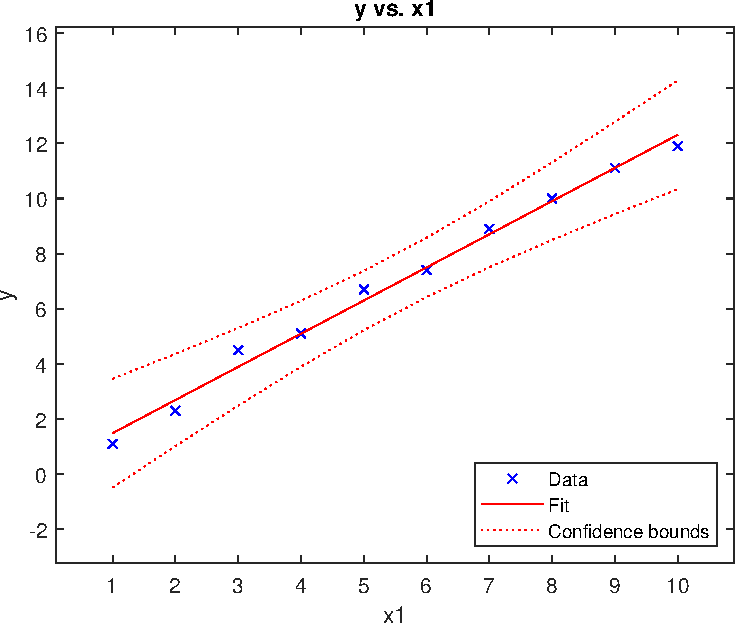
\includegraphics[width = \linewidth, keepaspectratio = true]{figures/linear_regression.pdf}
    \caption{Graph of linear regression model.}
    % \label{}
\end{figure}
Note that:
\begin{itemize}
    \item The confidence band is narrowest at \(x = \overline{x}\).
    \item More than \(95\%\) of observations fall outside the confidence band because that interval is based on the expected value not specific observations.
    \item As the confidence band widens further away from \(\overline{x}\), extrapolation beyond the range of known \(x\) values is dangerous.
\end{itemize}
\begin{proof}
    To prove the standard error \(s_{\hat{y}_i}\), we notice
    \begin{equation*}
        \hat{y}_i = \hat{\beta}_0 + x_i \hat{\beta}_1
    \end{equation*}
    This will allow us to represent the variance as
    \begin{align*}
        \Var{\left( \hat{y}_i \right)} & = \Var{\left( \hat{\beta}_0 + x_i \hat{\beta}_1 \right)}                                                                                    \\
                                       & = \Var{\left( \hat{\beta}_0 \right)} + x_i^2 \Var{\left( \hat{\beta}_1 \right)} + 2 x_i \Cov{\left( \hat{\beta}_0,\: \hat{\beta}_1 \right)}
    \end{align*}
    Then using the rules for covariance
    \begin{align*}
        \Cov{\left( \hat{\beta}_0,\; \hat{\beta}_1 \right)} & = \Cov{\left( \overline{y} - \overline{x} \hat{\beta}_1,\: \hat{\beta}_1 \right)}                                       \\
                                                            & = \Cov{\left( \overline{y},\: \hat{\beta}_1 \right)} - \Cov{\left( \overline{x} \hat{\beta}_1,\: \hat{\beta}_1 \right)} \\
                                                            & = - \overline{x} \Cov{\left( \hat{\beta}_1,\: \hat{\beta}_1 \right)}                                                    \\
                                                            & = - \overline{x} \Var{\left( \hat{\beta}_1 \right)}
    \end{align*}
    Therefore
    \begin{align*}
        \Var{\left( \hat{y}_i \right)} & = \Var{\left( \hat{\beta}_0 \right)} + x_i^2 \Var{\left( \hat{\beta}_1 \right)} - 2 x_i \overline{x} \Var{\left( \hat{\beta}_1 \right)} \\
                                       & = \Var{\left( \hat{\beta}_0 \right)} + x_i \Var{\left( \hat{\beta}_1 \right)} \left( x_i - 2 \overline{x} \right)                       \\
                                       & = s_{\hat{\beta}_0}^2 + x_i s_{\hat{\beta}_1}^2 \left( x_i - 2 \overline{x} \right)
    \end{align*}
    We can now substitute the known values for the variance from the previous sections.
    \begingroup
    \allowdisplaybreaks{}
    \begin{align*}
        \Var{\left( \hat{y}_i \right)} & = s^2 \frac{\sum_i^n x_i^2}{n\sum_i^n \left( x_i - \overline{x} \right)^2} + x_i s^2 \frac{1}{\sum_i^n \left( x_i - \overline{x} \right)^2} \left( x_i - 2 \overline{x} \right)    \\
                                       & = s^2 \left[ \frac{\sum_i^n x_i^2}{n \sum_i^n \left( x_i - \overline{x} \right)^2} + \frac{x_i^2 n - 2 \overline{x} x_i n}{n \sum_i^n \left( x_i - \overline{x} \right)^2} \right] \\
                                       & = s^2 \frac{\sum_i^n x_i^2 + x_i^2 n - 2 \overline{x} x_i n}{n\sum_i^n \left( x_i - \overline{x} \right)^2}                                                                        \\
                                       & = s^2 \frac{\sum_i^n \left( x_i^2 - 2\overline{x}x_i + 2\overline{x} x_i \right) + x_i^2 n - 2 \overline{x} x_i n}{n\sum_i^n \left( x_i - \overline{x} \right)^2}                  \\
                                       & = s^2 \frac{\sum_i^n \left( x_i^2 - 2\overline{x}x_i \right) + 2\overline{x} \sum_i^n x_i + x_i^2 n - 2 \overline{x} x_i n}{n\sum_i^n \left( x_i - \overline{x} \right)^2}         \\
                                       & = s^2 \frac{\sum_i^n \left( x_i^2 - 2\overline{x}x_i \right) + 2\overline{x}^2 n + x_i^2 n - 2 \overline{x} x_i n}{n\sum_i^n \left( x_i - \overline{x} \right)^2}                  \\
                                       & = s^2 \frac{\sum_i^n \left( x_i^2 - 2\overline{x}x_i + \overline{x}^2 \right) + \overline{x}^2 n + x_i^2 n - 2 \overline{x} x_i n}{n\sum_i^n \left( x_i - \overline{x} \right)^2}  \\
                                       & = s^2 \frac{\sum_i^n \left( x_i - \overline{x} \right)^2 + n \left( x_i - \overline{x} \right)^2}{n\sum_i^n \left( x_i - \overline{x} \right)^2}                                   \\
                                       & = s^2 \left[ \frac{1}{n} + \frac{\left( x_i - \overline{x} \right)^2}{\sum_i^n \left( x_i - \overline{x} \right)^2} \right]
    \end{align*}
    \endgroup
\end{proof}
\subsection{Coefficient of Determination}
The linear regression output also gives us the coefficient of determination labelled \(R^2\).
\begin{definition}[Coefficient of Determination]
    The coefficient of determination \(R^2\) describes the percentage of the observed variance
    in \(y\) that is explained by the fitted model \(\hat{y}\).
    \begin{equation*}
        R^2 = 1 - \frac{RSS}{TSS}
    \end{equation*}
    where \(RSS\) is the regression sum of squares defined
    \(\sum_i^n\left( \hat{y}_i - y_i \right)^2\) and \(TSS\) is the total sum
    of squares defined \(\sum_i^n \left( y_i - \overline{y} \right)^2\).
\end{definition}
This value is labelled \lstinline!R-squared! in the MATLAB output.
\section{Linear Regression Diagnostics}
After fitting a linear model, it is important to check that linearity is the best assumption for the relationship between the variables.

We can do this using a residual plot.
\subsection{Summary of Assumptions}
During the process of linear regression, we make a number of assumptions:
\begin{enumerate}
    \item Each observation is independent of other observations
    \item The relationship between \(X\) and \(Y\) is best modelled as a linear relationship
    \item The residuals are have a Normal distribution
    \item The variance of the residuals is constant for all observations
\end{enumerate}
\end{document}